\chapter{Trajectory Generator}\label{chap:trajectory_generator}
This section describes the module that computes the trajectory the vehicle has to execute to accompish the task of landing on a moving platform.\\

A trajectory is a sequence of desired states that leads the UAV from an initial condition at $t = t_0 $ to the desired final condition reached at $t = T$. In particular, a desired state at a certain time $t_i$ is defined as:
 \begin{itemize}
\item $[p_{x,t_i,des},p_{y,t_i,des},p_{z,t_i,des}]$: desired 3D position;
\item $[v_{x,t_i,des},v_{y,t_i,des},v_{z,t_i,des}]$: desired linear velocity;
\item $[a_{x,t_i,des},a_{y,t_i,des},a_{z,t_i,des}]$: desired linear acceleration;
\item $[\psi_{t_i,des}]$: desired yaw.
\end{itemize}
The fact that the desired state of the quadrotor is completely defined by these quantities is because the quadrotor dynamics are differentially flat \cite{van1997real}: the states and the inputs can be written as algebraic functions of four flat outputs and their derivatives: $[x,y,z,\psi]$.\\

The initial desired state, for $t_i = t_0$, is given by the state estimation of the quad, while the final condition for $t_i = T$ are given from the state machine module. \\

The final conditions can be of different types, and the calculation of the possible trajectories depends on them:
\begin{itemize}
\item During the first two stages of the state machine, the final state is simply a pose in the world frame with zero velocity and acceleration. This module computes some trajectories from the initial state to this final states with different total times $T_i$ and it is choosing the one that is minimizing a specific cost function. We will see in the following sections, the different cost functions that can be chosen.\\ 
The times $T_i$ depend on the distance between initial and final position, and the average velocity that the quad should have during the flight.
\item During the third stage, the final state is a pose in the world frame with a velocity equal to the one of the moving platform, and zero acceleration. The module calculates the trajectories like in the previous case, so for different times $T_i$, and picks the best option.
\item When the UAV has to align and land on the base, the state machine provides to the trajectory generator a set of possible final states with positions $p_i$, velocities $v_i$ and times $T_i$ to reach them. This module calculates all the trajectories to reach all these possible final conditions in the correspondent time, and chooses the best one.
\end{itemize}
Note that the choice of the final trajectory among all the possible calculates is done with respect to a cost function that will be discuss later.

\begin{figure}[!htbp]
    \centering
    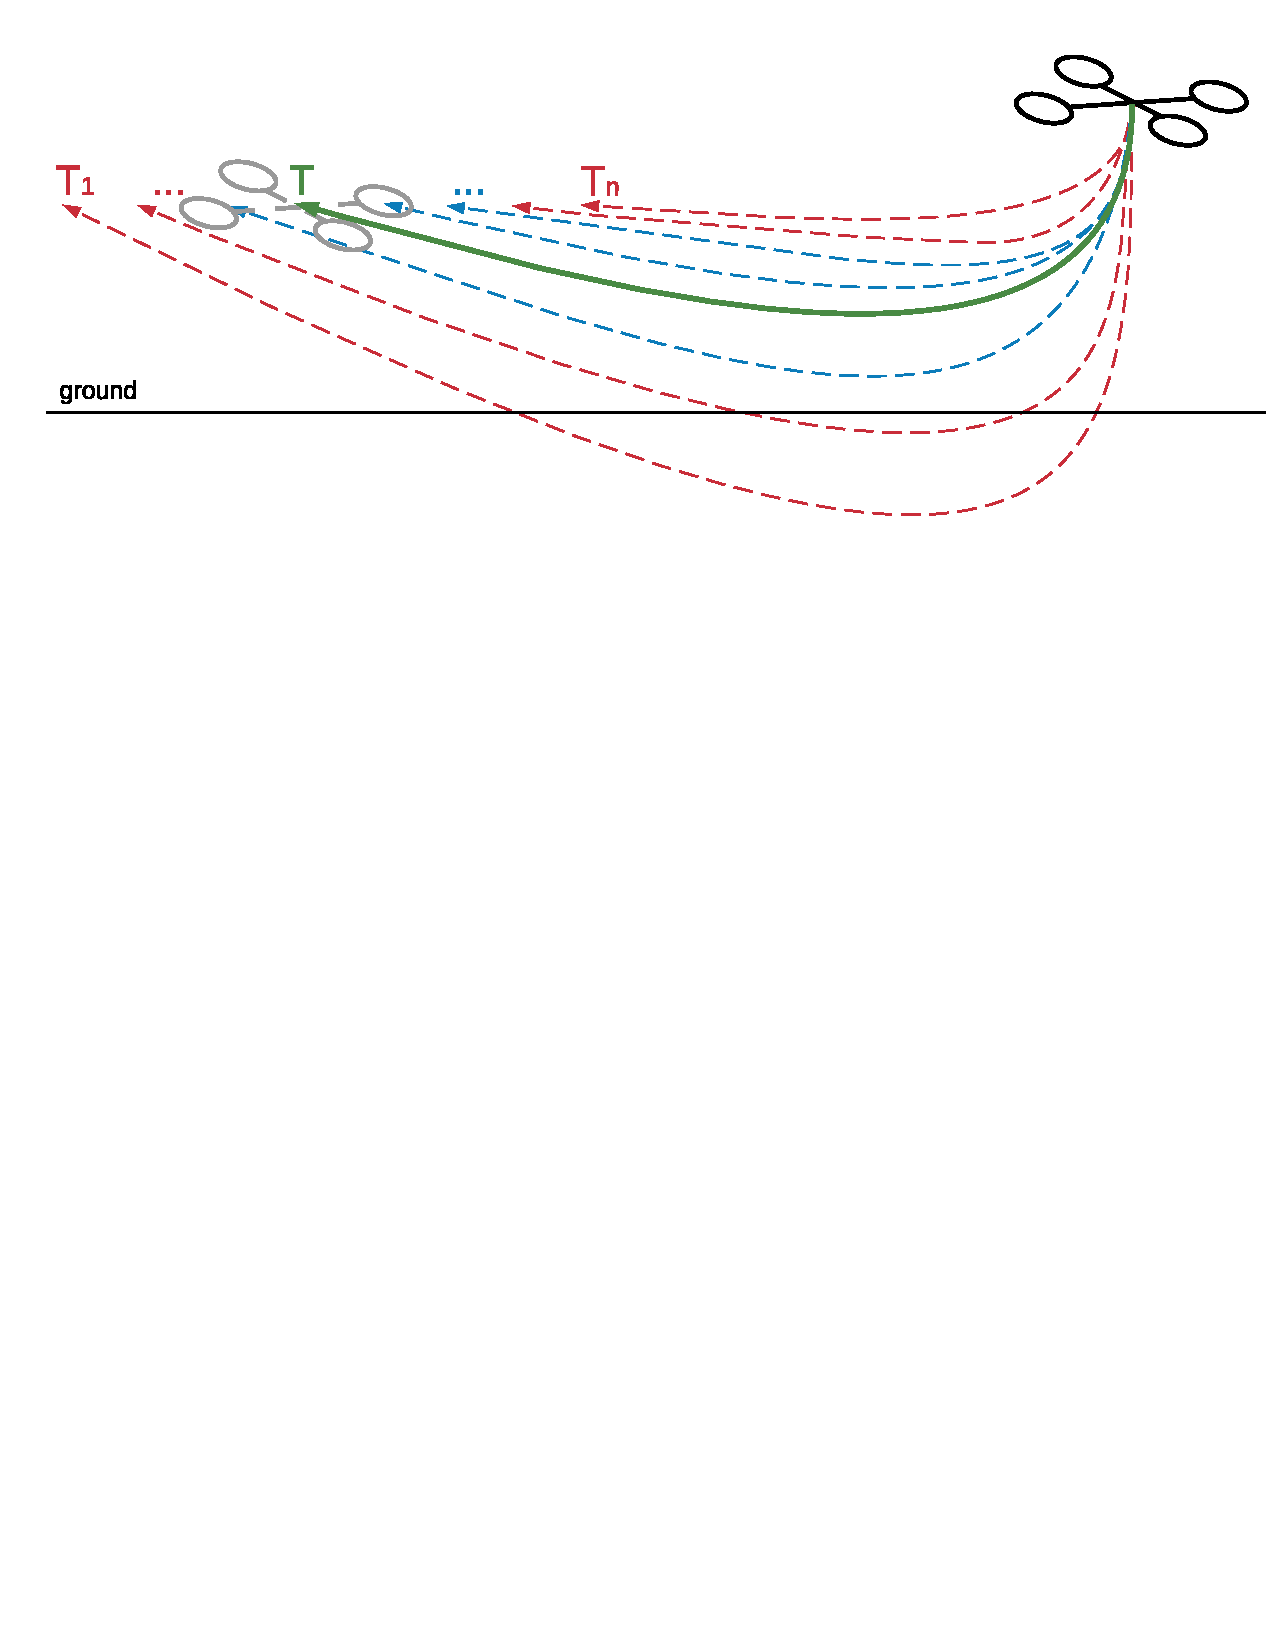
\includegraphics[width=0.8\textwidth]{img/trajectory_generation.pdf}
    \caption{The scheme synthesizes the concept of multiple possible trajectory generated and then pick the best one. The red trajectory are unfeasible (state or input unfeasible), the green trajectory is the best solution found.}
    \label{fig:traject_gen}
\end{figure}

The trajectory planning module is constituted by two threads:
\begin{itemize}
\item The first thread is popping and publishing the top of a stack of desired states with rate $r_{trj}$. This state will be the input of the high controller module.
\item The second thread:
\begin{itemize}
\item receives the initial and final conditions;
\item checks if these two belong to the previous trajectory (within an error), and only if they do not, proceed with the following tasks;
\item calculates the best trajectory;
\item samples the trajectory with a given rate $r_{trj}$;
\item substitutes the desired states inside the stack of the first thread with the new samples.
\end{itemize}
\end{itemize}

\begin{figure}[!htbp]
    \centering
    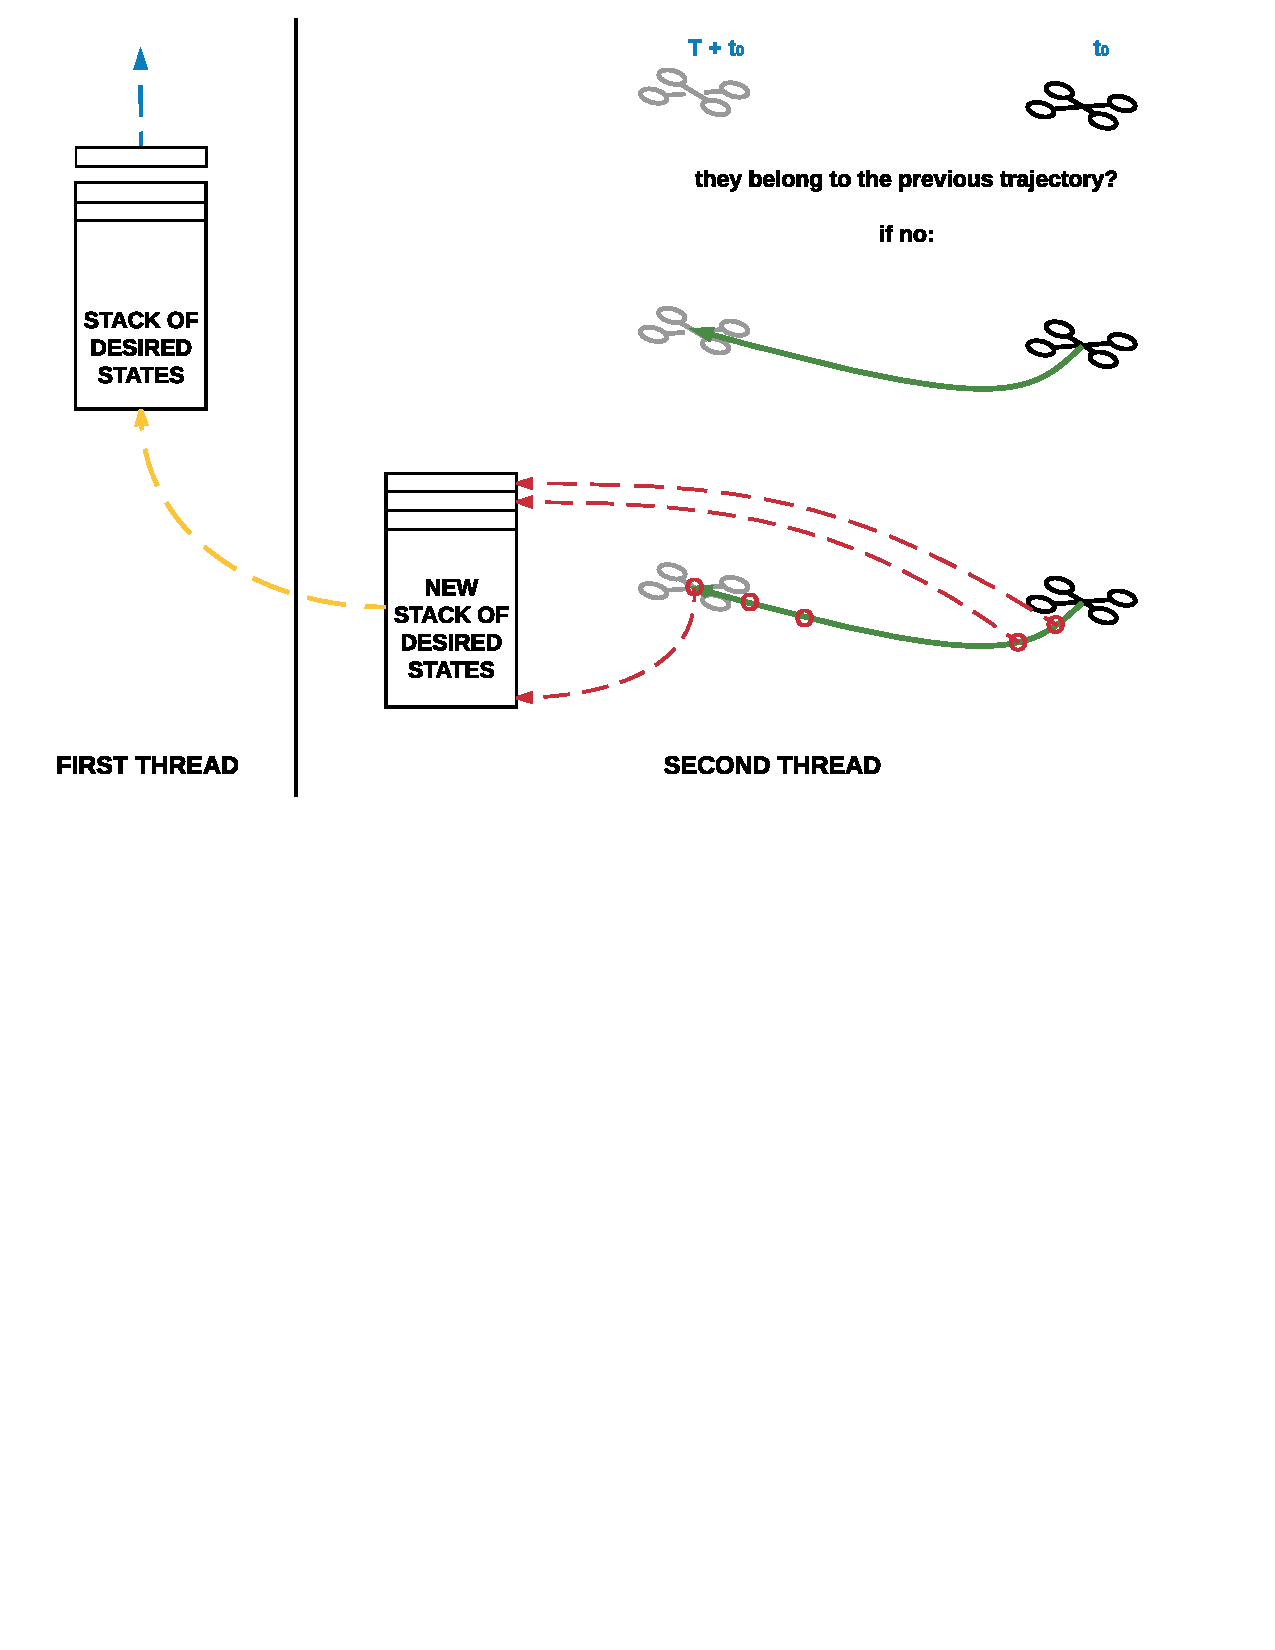
\includegraphics[width=1.0\textwidth]{img/threads_trajectory_generation.pdf}
    \caption{Scheme of tasks subdivision between the two threads.}
    \label{fig:traject_gen}
\end{figure}

In this module, we utilize the trajectory planning approach described in \cite{mueller2015computationally} to generate thousands of trajectories per second (\SI{2}{\milli \second} each), and then choose the best one to follow. We do this calculation with frequent replanning in order to correct any errors related to the prediction of the final target or related to a displacement between desired state and actual state of the quadrotor, due to the not perfect tracking of the trajectory by the controller.\\

\section{Minimum jerk trajectory}
The algorithm proposed in \cite{mueller2015computationally} produces trajectories that are the result of an optimal control problem with the goal of computing a thrice differentiable trajectory which guides the quadrotor from an initial state (position, velocity, acceleration and yaw of the UAV) to a final state in a finite time $T$, while minimizing a cost function that can be considered as an upper bound on the average of a product of the inputs to the quadrotor system.\\ Furthermore, the final trajectory takes in account feasibility with respect to input and space constraints.
\subsection{Dynamic Model}
Consider the classic simplified dynamic model of the quadrotor:
\begin{align}
\begin{cases}
\ddot{\boldsymbol{r}} = \boldsymbol{g} + \boldsymbol{R}_{WB}\boldsymbol{c}  \\[10pt]
\dot{\boldsymbol{R}}_{WB} = \boldsymbol{R}_{WB}\hat{\boldsymbol{w}_{WB}}
\end{cases},
\label{eq:dynamic_jerk}
\end{align}
where 
\begin{align}
\hat{\boldsymbol{w}_{WB}} =
{\begin{bmatrix}
0 & -\omega_3 & \omega_2 \\[10pt]
\omega_3 & 0 & -\omega_1 \\[10pt]
-\omega_2 & \omega_1  & 0
\end{bmatrix}} \ \ \ \ \ \ \boldsymbol{c} = 
{\begin{bmatrix}
0 \\[10pt]
0 \\[10pt]
c
\end{bmatrix}} = \boldsymbol{e}_3c.
\label{eq:52}
\end{align}
In \eqref{eq:52} input are  $c$, the total normalized thrust, and the angular rates $\omega_1,\omega_2,\omega_3$. Now the goal is to express these inputs in function of the states and the jerk.
 
The input thrust $c$ is computed by applying the norm to the position dynamics:
\begin{align}
c^2 &= ||\boldsymbol{c}||^2 =  ||\ddot{\boldsymbol{r}} - \boldsymbol{g}||^2, \\[20pt] \label{eq:thrust_from_jerk}
\begin{split}
2c\dot{c} &= 2(\ddot{\boldsymbol{r}} - \boldsymbol{g})^T \boldsymbol{j} = 2 c\boldsymbol{e}_3^T\boldsymbol{R}_{WB}^T \boldsymbol{j}  , \\[10pt]
\dot{c} &= \boldsymbol{e}_3^T\boldsymbol{R}_{WB}^T \boldsymbol{j} .
\end{split}
\end{align}

We can also define the position dynamics in therms of jerk:
\begin{align}
\boldsymbol{j} &= \dddot{\boldsymbol{r}} = \dot{\boldsymbol{R}}_{WB}\boldsymbol{c} + \boldsymbol{R}_{WB}\dot{\boldsymbol{c}}.
\end{align}

Combining the two derivations, we can say that fixed $\boldsymbol{j}$ and $c$, we define uniquely two components of the body rates:
\begin{align}
{\begin{bmatrix}
\omega_1 \\[10pt]
\omega_2
\end{bmatrix}}  = \frac{1}{c}
{\begin{bmatrix}
1 & 0 & 0  \\[10pt]
0 & 1 & 0
\end{bmatrix}}\boldsymbol{R}_{WB}^T \boldsymbol{j}
\label{eq:omega_from_jerk}
\end{align}
Using these equations the inputs of the system are defined with a degree of freedom in $\omega_3$.\\

The goal of this algorithm is to find  the trajectory $\boldsymbol{z}(t)$ for $t \in [0,T]$, consisting of the quadrotor position, velocity and acceleration, such that:
\begin{align}
\boldsymbol{z}(t) = (\boldsymbol{r}(t),\dot{\boldsymbol{r}}(t),\ddot{\boldsymbol{r}}(t)) \in \mathbb{R}^9
\end{align}
with given initial and final conditions $\boldsymbol{z}(0)$ and $\boldsymbol{z}(T)$.

If we consider the system input to be the three-dimensional jerk, then we can decouple the dynamics into three orthogonal inertial axes, and treat each axis as a triple integrator with jerk used as control input. The true control inputs $c$ and $\boldsymbol{\omega}$ are then recovered from $\boldsymbol{j}$  using \eqref{eq:thrust_from_jerk} and \eqref{eq:omega_from_jerk}.


\subsection{Optimal control problem}
The trajectory generation is rewritten as a discrete optimal control problem, with boundary conditions defined by the quadrotor initial and (desired) final states. The solution of this problem must minimize a cost function subject to some dynamics and satisfying state and inputs conditions.\\

As we said, the dynamics are split among the three decoupled axis, and for each axis the optimal control problem is  solved independently. For a single axis the problem is defined as follows. Find the sequence of control input $j_k$ that minimizes:
\begin{align}
J = \sum_{k=0}^{N-1} j_k^2,
\end{align}

subject to the dynamics:
\begin{align}
\begin{split}
j_k &= \dddot{r}_k,\\[10pt]
z_k  &= 
{\begin{bmatrix}
 r_k \\[5pt]
 \dot{r}_k \\[5pt]
 \ddot{r}_k
\end{bmatrix}} = 
{\begin{bmatrix}
1 & dt & \frac{dt^2}{2}  \\[5pt]
0 & 1 & dt \\[5pt]
0 & 0 & 1
\end{bmatrix}}z_{k-1} + 
{\begin{bmatrix}
 \frac{dt^3}{6}  \\[5pt]
 \frac{dt^2}{2} \\[5pt]
 dt
\end{bmatrix}}j_{k-1}, \\[10pt]
z_0 &= z(0), \\[5pt]
z_N &= z(T),
\end{split}
\end{align}
and respecting the constraints:
\begin{align}
A
{\begin{bmatrix}
 r_k \\[10pt]
j_k
\end{bmatrix}} \leq b.
\end{align}

The solution of this optimal control problem can be found in close form with Pontryagin's minimum principle.
In the paper \cite{mueller2015computationally} are presented all the calculations to derive the solution. The final result requires the evaluation of a single matrix that depends on the initial and final condition $z(0)$ $z(T)$ and the total time $T$.

\subsection{Cost function}
The cost function selected is, considering the three axis together:
\begin{align}
J = \sum_{k=0}^{N-1} ||\boldsymbol{j}_k||^2
\end{align}

This cost function has been chosen because it can be interpreted as an upper bound for a product of the input (using \eqref{eq:omega_from_jerk}):
\begin{align}
c_k^2||\boldsymbol{\omega}_k||^2 = \Big|\Big| c_k
\begin{bmatrix}
\omega_{1,k} \\[2pt]
\omega_{2,k}
\end{bmatrix}\Big|\Big|^2 = \Big|\Big| c_k \frac{1}{c_k}
{\begin{bmatrix}
1 & 0 & 0  \\[2pt]
0 & 1 & 0
\end{bmatrix}}\boldsymbol{R}_{WB,k}^T \boldsymbol{j}_k\Big|\Big|^2 \leq ||\boldsymbol{j}_k||^2
\end{align}

\subsection{Constraints}
The trajectory is feasible if $c$ and $||\boldsymbol{\omega}||$ respect the following conditions for all t of the trajectory:
\begin{align}
\begin{split}
0 < c_{min} \leq c &\leq c_{max},\\
||\boldsymbol{\omega}|| & \leq \omega_{max}.
\end{split}
\end{align}

These constraints can be rewritten in therm of the state and the jerk. For the thrust
\begin{align}
\begin{split}
 c_{min}^2 \leq c^2 &\leq c_{max}^2,\\
 c_{min}^2 \leq ||\ddot{\boldsymbol{r}} - \boldsymbol{g}||^2 &\leq c_{max}^2.\\
\end{split}
\label{eq:feasib_thrust}
\end{align}
For the body rates:
\begin{align}
\begin{split}
||\boldsymbol{\omega}|| =
 {\begin{bmatrix}
\omega_1 & \omega_2
\end{bmatrix}}
 {\begin{bmatrix}
\omega_1 \\[10pt]
\omega_2
\end{bmatrix}} + \omega_3^2 = {\begin{bmatrix}
\omega_1 & \omega_2
\end{bmatrix}}
 {\begin{bmatrix}
\omega_1 \\[10pt]
\omega_2
\end{bmatrix}}  \leq \frac{1}{c}||\boldsymbol{j}||  \leq \omega_{max} 
\end{split}
\label{eq:feasib_bodyrates}
\end{align}
where we assume $\omega_3 = 0$

\subsection{Feasibility check} \label{feasibility_check}
A fast conservative verification is applied to check the feasibility of the trajectory. For the thrust, from \eqref{eq:feasib_thrust}, we know that the trajectory is unfeasible if:
\begin{align}
\max_{k=[0,N]} {(\ddot{r}_{i,k}- \delta_{i,z}g)^2} > c_{max}^2 \ \ \ \ \forall i\in\{x,y,z\}, \\
\min_{k=[0,N]} {(\ddot{r}_{i,k} -\delta_{i,z}g)^2} < c_{min}^2 \ \ \ \ \forall i\in\{x,y,z\},
\end{align}
where $\delta_{i,z}$ is equal to $1$ if $i=z$ (we are considering the $z$ axis) otherwise it is $0$.\\
On the other hand the trajectory is definitely feasible if:
\begin{align}
\sum_i{\max_{k=[0,N]} {(\ddot{r}_{i,k}-  \delta_{i,z}g)^2}} \leq c_{max}^2 \ \ \ \ i\in\{x,y,z\},\\
\sum_i{\min_{k=[0,N]} {(\ddot{r}_{i,k} -  \delta_{i,z}g)^2}} \geq c_{min}^2 \ \ \ \  i\in\{x,y,z\}.
\label{eq:thrust_minmax}
\end{align}
If both these checks fail, the trajectory is considered interminable.\\

For the body rates, from \eqref{eq:feasib_bodyrates} we know that the trajectory is feasible only if:
\begin{align}
\ddfrac{\sum\limits_{i=1} \  \max\limits_{k=[0,N]} j_{i,k}^2 }{\sum\limits_{i=1} \ {\min\limits_{k=[0,N]} {(\ddot{r}_{i,k} -  \delta_{i,z}g)^2}}} \leq \omega_{max} \ \ \ \ i\in\{x,y,z\}
\label{eq:body_rates_max}
\end{align}

If the trajectory is indeterminable, then the feasibility checks are repeated separately in the two sub intervals $[1,\frac{N}{2}], [\frac{N}{2}+1,N]$, iteratively. The check stops when all the subset are feasible, or one is unfesible, or if the subdivision has arrived at intervals smaller than a certain threshold.


\subsection{Estimating the acceleration} \label{subsec:acceleration}
The trajectory generation method we used in this work needs an initial and a final state. The initial state is always selected as the current position velocity and acceleration of the quadrotor. From the state estimate of MSF we have the first two information, while the third has to be estimated separately.\\
There are several ways to obtain this estimate:
\begin{itemize}
\item IMU: the Inertial unit gives measurements of the 3D linear accelerations of the vehicle. This measures are noisy when the quadrotor is flying because of the motors vibrations. This renders necessary to filter the measure with a low pass:
 \begin{align}
a_{imu}(t_k) = \Big(1-e^{-\frac{t_k-t_{k-1}}{\tau_{a_{imu}}}}\Big)imu(t_k) + e^{-\frac{t_k-t_{k-1}}{\tau_{imu}}} a_{imu}(t_{k-1}).
\label{eq:imu_acc}
\end{align}
\item Finite difference: Having two successive velocity estimation we can calculate the acceleration approximating the derivative of the velocity with a numerical finite difference:
\begin{align}
\dot{v}(t_k) \simeq \frac{v(t_k)-v(t_{k-1})}{t_k-t_{k-1}},
\label{eq:finite_difference}
\end{align}
Also this method is really sensitive to high frequency noise, and the data must be filter with low pass filter:
 \begin{align}
a_{fd}(t_k) =  \Big(1-e^{-\frac{t_k-t_{k-1}}{\tau_{fd}}}\Big)\frac{v(t_k)-v(t_{k-1})}{t_k-t_{k-1}} + e^{-\frac{t_k-t_{k-1}}{\tau_{a_{fd}}}}. a_fd(t_{k-1})
\label{eq:finite_difference}
\end{align}
\item Thrust: from the equation of motion of the quadrotor we know that the acceleration of the UAV in a specific moment is completely described by the total thrust $\boldsymbol{c}$ applied and the rotation of the quadrotor $\boldsymbol{R}_{WB}$ :
\begin{align}
{\begin{bmatrix}
\ddot{x} \\[10pt]
\ddot{y} \\[10pt]
\ddot{z}
\end{bmatrix}}=
{\begin{bmatrix}
0 \\[10pt]
0 \\[10pt]
-g
\end{bmatrix}} 
+ \boldsymbol{R}_{WB}
{\begin{bmatrix}
0 \\[10pt]
0 \\[10pt]
c
\end{bmatrix}}.
\end{align}
Also, we know that:
 \begin{align}
c = \frac{1}{m}\sum_{i=1}^{4}{f_i},
\end{align}
where $f_i$ is the thrust produced by the $i$-th propeller.\\
From the low level controller Eq~\eqref{eq:thrusts} we have these values, and so we can calculate the acceleration vector. It is important to notice that the information from the low level control are the desired thrust for each propeller $\tilde{f}_i$, not the actual one $f_i$. The real produced thrust can be calculated as $\lambda_i\tilde{f}_i$ where $\lambda_i$ is the rotor fitness coefficients. These coefficients are estimated in hover conditions before starting the mission.
\end{itemize}

In the final implementation we decided to use the thrust that, even if it shows some offset in the z direction (see Sec.~\ref{subsec:acceleration_experiments} for more details) with respect to the other two methods, is more smooth and does not need a filtering.


\section{Minimum snap trajectory}
When the minimum snap trajectory algorithm fails to find a feasible trajectory, and no previous trajectories are available, we have to find another way to calculate the sequence of desired states.\\
If this is the case, we use a minimum snap trajectory \cite{mellinger2011minimum}. This type of trajectories are the solution of another optimization problem in which the inputs are expressed in function of the fourth derivative of the position, namely the snap.\\

The problem formulation uses a more complete dynamics of the quad with respect to the jerk formulation \eqref{eq:dynamic_jerk}
:
\begin{align}
\begin{cases}
\ddot{\boldsymbol{r}} = \boldsymbol{g} + \boldsymbol{R}_{WB}\boldsymbol{c}  \\[10pt]
\dot{\boldsymbol{R}}_{WB} = \boldsymbol{R}_{WB}\hat{\boldsymbol{w}_{WB}}  \\[10pt]
\dot{\boldsymbol{w}}_{WB} = J^{-1} (\boldsymbol{\tau} - \boldsymbol{w}_{WB} \times J\boldsymbol{w}_{WB})
\end{cases}
\end{align}
where $\boldsymbol{\tau}$ are the torques acting on the body causated by the totor thrust \eqref{eq:torques}.\\

Using these dynamics we need a derivative more in order to express the input in therms of the flat outputs.
Because of that, the states must be described as position, velocity, acceleration and jerk. \\
In order to compute this type of trajectory we should calculate the initial jerk, but since it is difficult to estimate its value we set the initial and final jerks to be zero, while the other values of the initial condition are calculated as the previous section's algorithm.\\

In this new formulation, the optimization problems minimizes the following cost function:
\begin{align}
J = \sum_{k=0}^N\Big( \mu_r \Big|\Big|\frac{d^{4}\boldsymbol{r}_k}{dt^{4}}\Big|\Big|  +  \mu_{\psi} \Big|\Big|\frac{d^{2}\boldsymbol{\psi}_k}{dt^{2}}\Big|\Big|\Big).
\end{align}
%that is minimizing the snap (because the thrust and pitch and roll body rates are expressed as functions of the forth derivative of the position $\boldsymbol{r}$), and the yaw angular acceleration for minimizing the input relative (in the paper  \cite{mellinger2011minimum} there are all the calculations to express the inputs as function of the snap).

Since this problem does not have a close form, it is written as a quadratic program:
\begin{align}
\begin{split}
min & \ \ \boldsymbol{x}^T\boldsymbol{H}\boldsymbol{x} + \boldsymbol{h}^T\boldsymbol{x},\\[10pt]
s.t. &\ \ \boldsymbol{Ax} \leq \boldsymbol{b}
\end{split}
\end{align}
and then solved with optimization algorithms, finding numerically the result.\\ 

This problem requires, on average, more time to be solved (\SI{20}{\milli \second}) with respect to the minimum jerk method, so it is not possible to generate multiple trajectories and select the best one at each control loop.\\

What we are do is calculating this trajectory taking, among all the final conditions that the state machine is given as input to this module, the one with longest time $T$ and so producing the trajectory of $T_{max}$ seconds from the initial state to this point, because, usually, the longer is the time $T$ the less aggressive must be the trajectory to reach the final state, so it is more probable that this trajectory we are calculating is feasible .

\section{Trajectory generation issues} \label{sec:trajectory_problem}
The trajectory generator previously described presents some issues that must be solved. In the following we report the main ones together with possible solutions.

\subsection{Last chance solution}
If both rapid trajectory and minimum snap trajectory do not find a feasible solution we apply this final method.\\

This method uses the rapid trajectory algorithm calculated with a final time $T_{feasible}$ such that the trajectory is surely feasible. In the paper \cite{mueller2015computationally} there is a method to calculate $T_{feasible}$ for a trajectory from rest to rest states (initial e final velocity and accelerations equal to 0).\\
In our case, the initial state can also be not static, so the solution should not hold in our case. What we can do is to enlarge the time $T_{feasible}$, from rest to rest, by a factor $\alpha$ proportional to the initial acceleration and velocity, and using this final time to calculate the rapid trajectory.\\

The minimum time $T_{feasible}$ is defined as the maximum between three different final times. The 3 times are calculate to guarantee the maxim thrust feasibility $T_{c_{max}}$, the minimum thrust feasibility $T_{c_{min}}$ and the body rates feasibility $T_{\omega_{max}}$. \\

We take 
\begin{align}
T_{feasible} = \alpha \max{(T_{c_{max}},T_{c_{min}},T_{\omega_{max}})},
\end{align}
because if  we calculate a feasible trajectory $trj_1$, from static to static states, with terminal time $T_1$, and then we calculate $trj_2$ with $T_2 \geq T_1$ as new terminal time, then the second trajectory will be surely feasible (this is not always true if initial and final conditions are not resting).\\

The parameters necessary to find these times are the distance $d$ between initial and final position, $c_{min}$, $c_{max}$ the minimum and maximum thrust, and $\omega_{max}$ the maximum body rates.\\ 
Substituting these variables into the general solution of the optimal control problem, calculating the maximum acceleration that the final trajectory will have, and using Eqs. \eqref{eq:thrust_minmax} and \eqref{eq:body_rates_max}, we can find the thee values of time:
\begin{align}
T_{c_{max}} &= \sqrt{\dfrac{10d}{\sqrt{3}(g-c_{min})}} \\[10pt]
T_{c_{min}} &= \sqrt{\ddfrac{10d}{\sqrt{3}(c_{max}-g)}} \\[10pt]
T_{\omega_{max}} &= \sqrt[3]{\ddfrac{60d}{\omega_{max}c_{min}}}
\end{align}

At this point, we can calculate the trajectory between the initial and final position with time duration $T_{feasible}$. This trajectory is considered a temporal solution, so as soon as a new initial or final condition arrive, we try to substitute it with a new trajectory. \\

Note that the solution found with this last method could not lead to the correct completion of the task in the last two parts of the state machine. In these phases the quadrotor must be in a precise amount of time $T$ in a specific position, in order to intersect the moving platform, while we are now considering a trajectory with duration $ T_{feasible} \neq T$.


%\subsection{Too frequent replanning}
%The main drawback of the algorithm used is that, in theory, it is possible to replan the trajectory at each control loop: in a MPC style, at each cycle, we calculate a trajectory from the initial state state to the final one and communicate just the first desired state to the high level control, repeating this procedure at the next loop.\\
%In practice, using this algorithm, the continuous replanning is not possible: when we pass the first desired state at the high controller the difference in position, velocity and acceleration are too tiny to actually generate a response from the quadrotor and start a movement. The outcome of this process is that the UAV does not move, as it should, and at the following control cycle the initial condition are only slightly changed, so the quadrotor results static in the initial position.\\
%
%This behaviour usually does not happen when we have to perform a trajectory in which the altitude is decreasing (small thrust required), but it is a great issue when the $z$ position should remain equal or increasing.\\
%This is why we do not perform a replan at each loop but only when it is necessary so when the final desired state has changed or the quadrotor is not tracking the trajectory.
%
%\begin{figure}[!htbp]
%    \centering
%    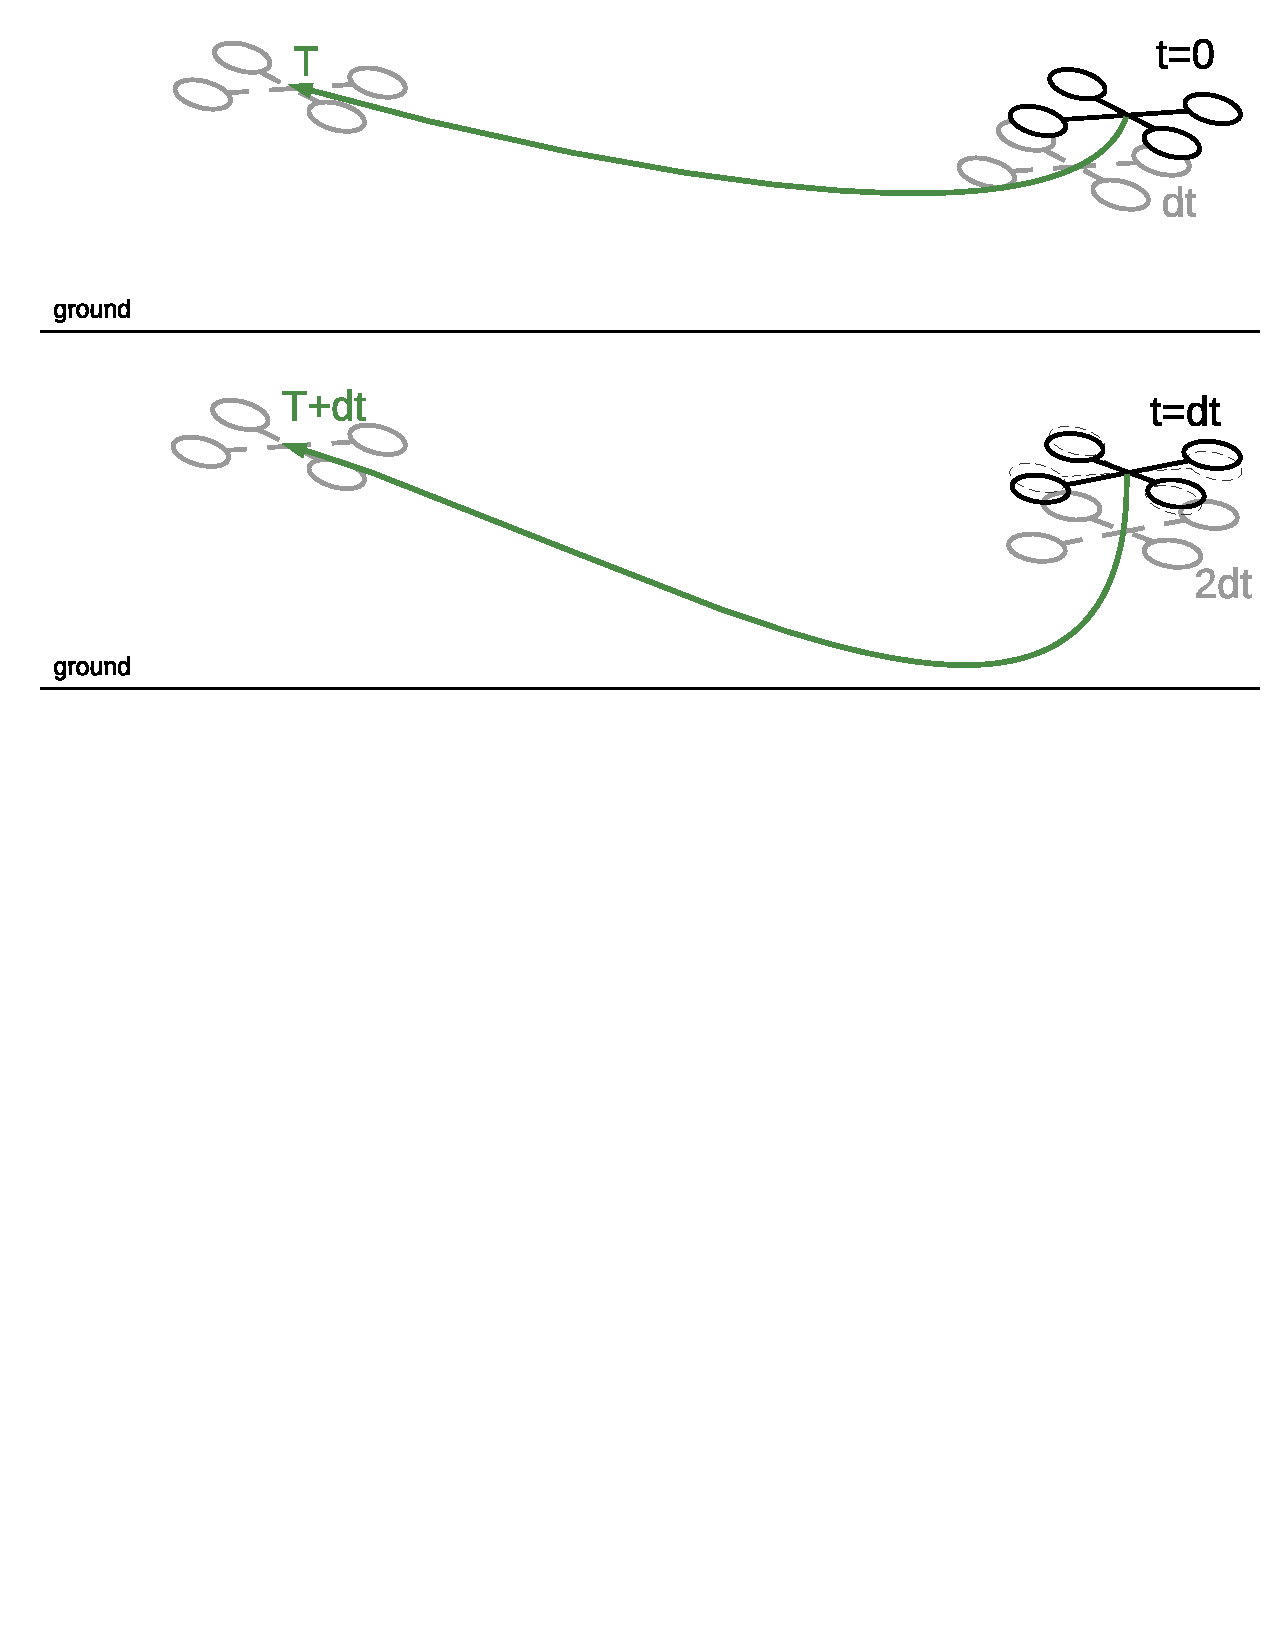
\includegraphics[width=0.7\textwidth]{img/frequent_replanning.pdf}
%    \caption{The scheme synthesizes the concept too frequent replanning. The quadrotor at time $dt$ should be in a position but the controller are not able to bring the UAV there. At the next loop the state of the quad is almost not changed, so it remains fixed in its initial state.}
%    \label{fig:freq_replan}
%\end{figure}


\subsection{Too short final time}
The rapid trajectory algorithm has another issue: when the final time $T$ is too short, all the calculated trajectories result indeterminable. This problem is due to the method used to check the feasibility with respect to the input, \ref{feasibility_check}, but to overcome this problem we can reduce the threshold for which the algorithm stop to recursively control if a piece of the trajectory is feasible.\\
This way the generation of the trajectory is slower, but we are able to find feasible trajectories when their duration is short.

